\subsection{Γωνία έναυσης 67 μοίρες για L=0.04Η και L=0.08Η}

\subsubsection{Τάση εξόδου}

\begin{figure}[h]
	\centering
	\begin{subfigure}{.5\textwidth}
		\centering
		\includegraphics[width = 0.9\linewidth]{Images/3_Vout_67_04}
		\caption{a = 67, L = 0.04}
		\label{fig:3_vout_67_04}
	\end{subfigure}%
	\begin{subfigure}{.5\textwidth}
		\centering
		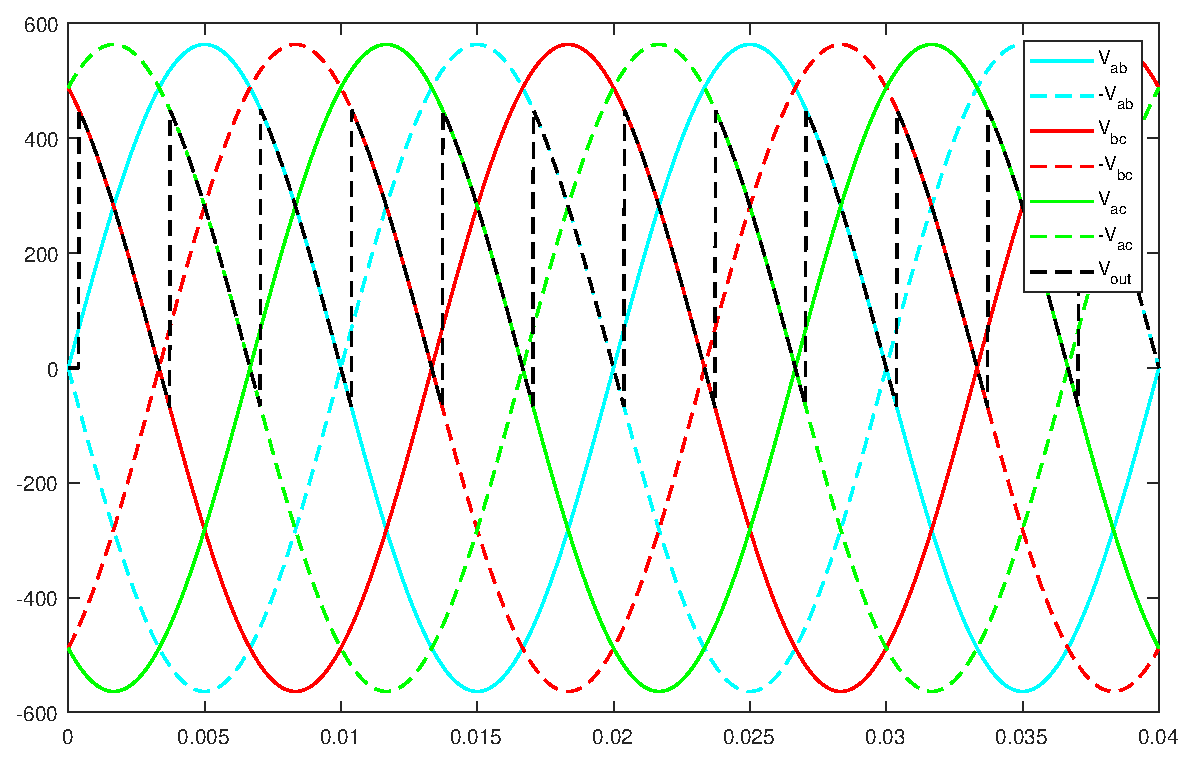
\includegraphics[width = 0.9\linewidth]{Images/3_Vout_67_08}
		\caption{a = 67, L = 0.04}
		\label{fig:3_vout_67_08}
	\end{subfigure}
	\caption{$V_{out} $ vs $V_{in}$ (a=0 L=0.04/0.08)}
	\label{figs:3_vout_67}
\end{figure}

\noindent
Έχοντας θέσει την γωνία έναυσης ίση με 67, τα thyristor πλέον άγουν με καθυστέρηση 67 μοιρών. 
Η γωνία έναυσης έχει ως αποτέλεσμα η τάση να μην ακολουθεί πλέον την μέγιστη τιμή. Επίσης, εφόσον η γωνία έναυσης είναι μεγαλύτερη από 60 μοίρες, η τάση πλέον παίρνει και αρνητικές τιμές καθώς τα thyristor καθυστερούν τόσο. Όσον αφορά την αύξηση της αυτεπαγωγής L, δεν παρατηρείται κάποια μεταβολή στις τάσεις καθώς όπως προαναφέρθηκε και στην ενότητα \ref{}, η τάση εξόδου είναι ανεξάρτητη της αυτεπαγωγής. Τέλος. λόγω της μεγαλύτερης γωνίας έναυσης, η μέση τιμή της τάσης έχει μειωθεί αρκετά και επίσης υπάρχουν πολλές διακυμάνσεις σε αυτή.,

\subsubsection{Ρεύμα εξόδου}

\begin{figure}[h]
	\centering
	\begin{subfigure}{.5\textwidth}
		\centering
		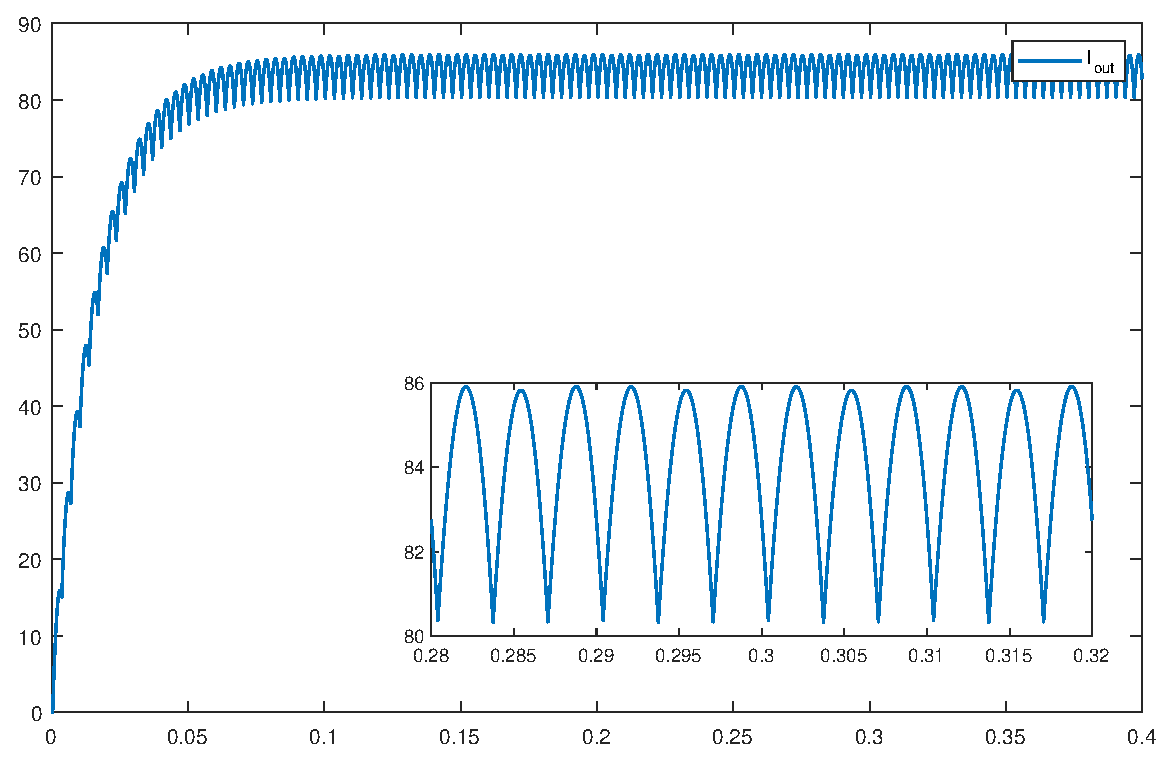
\includegraphics[width =1\textwidth]{Images/3_Iout_67_04}
		\caption{a = 67, L = 0.04}
		\label{fig:3_iout_67_04}
	\end{subfigure}%
	\begin{subfigure}{.5\textwidth}
		\centering
		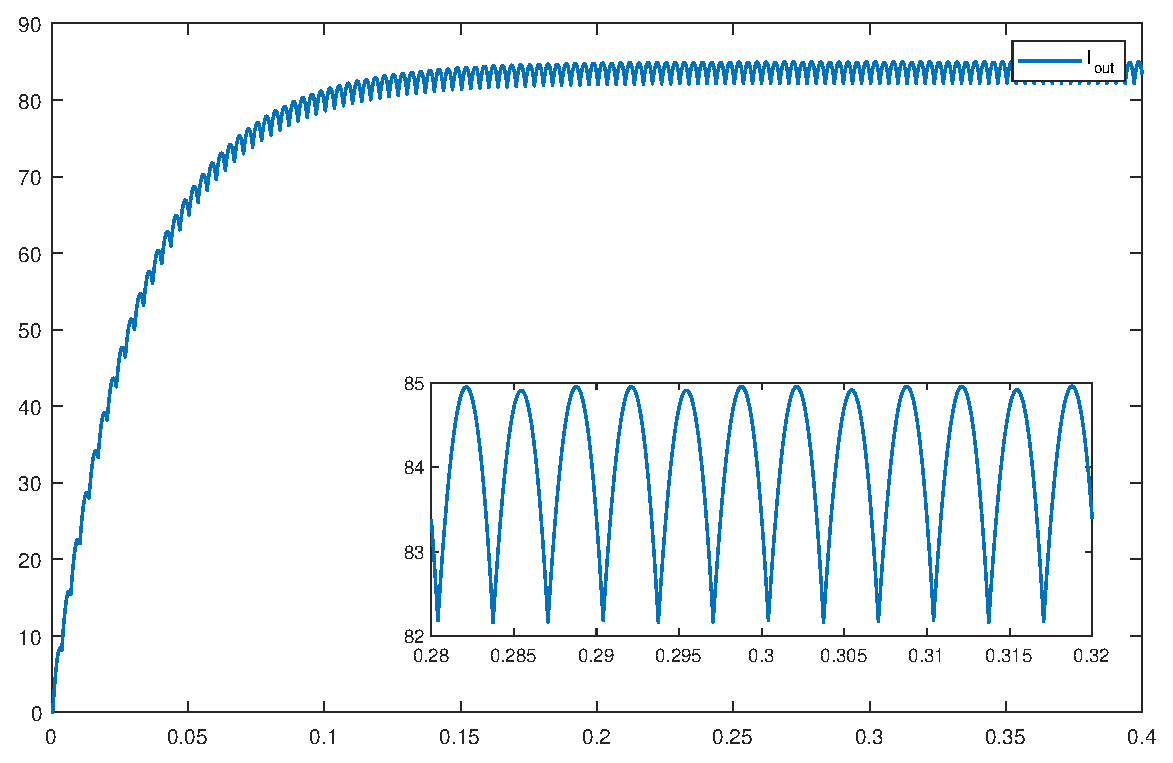
\includegraphics[width = 1\textwidth]{Images/3_Iout_67_08}
		\caption{a = 67, L = 0.04}
		\label{fig:3_iout_67_08}
	\end{subfigure}
	\caption{$I_{out} $ (a=67 L=0.04/0.08)}
	\label{figs:3_iout_67}
\end{figure}

Όσον αφορά το ρεύμα εξόδου, όπως στην υποενότητα \ref{}, για αύξηση της αυτεπαγωγής από 0.04 σε 0.08 H, το ρεύμα αργεί περισσότερο να σταθεροποιηθεί όμως παρουσιάζει μικρότερες διακυμάνσεις. Ωστόσο, να σημειωθεί πως το σήμα εξόδου του figure \ref{fig:3_iout_0_08}  προσομοιάζει πολύ καλύτερα το DC σε σχέση με το ρεύμα εξόδου του figure \ref{fig:3_iout_67_08}. Η διακυμάνσεις αυτές οφείλονται στη μεγάλη γωνία έναυσης και εφόσον αυτή είναι αρκετά μεγάλη, το ρεύμα μειώνεται σημαντικά εως ότου άγει το επόμενο thyristor και αρχίσει να αυξάνεται εκ νέου. 
\clearpage

\subsubsection{Ρεύμα Thyristor}
\begin{figure}[h]
	\centering
	\begin{subfigure}{.5\textwidth}
		\centering
		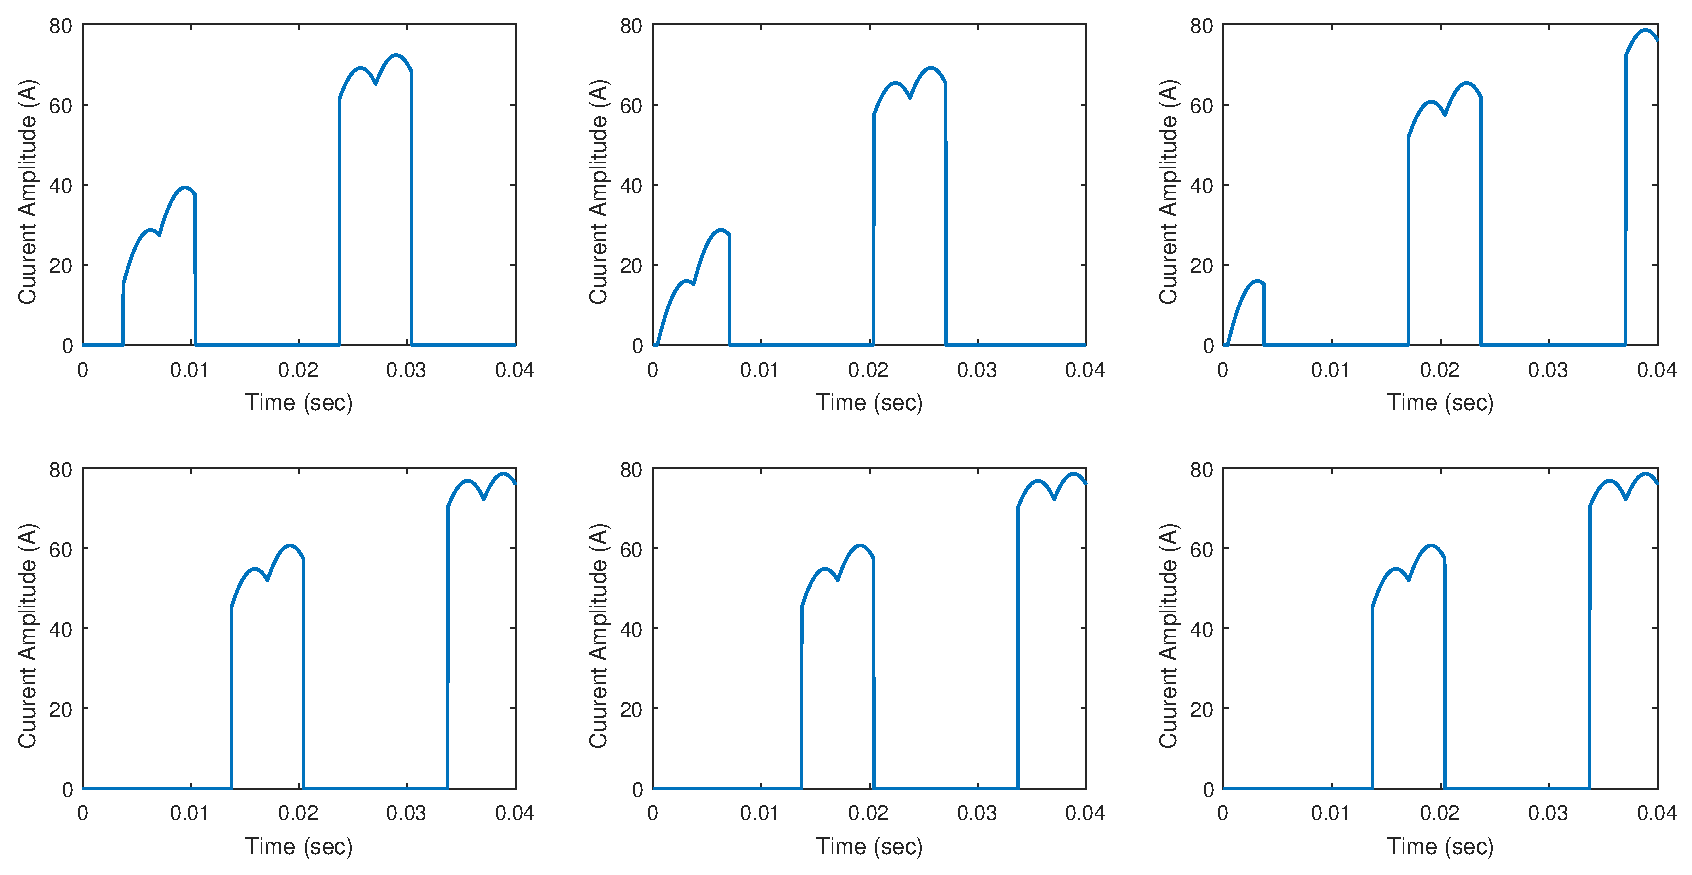
\includegraphics[width =0.9\textwidth]{Images/3_ThI_67_04}
		\caption{a = 67, L = 0.04}
		\label{fig:3_ThI_67_04}
	\end{subfigure}%
	\begin{subfigure}{.5\textwidth}
		\centering
		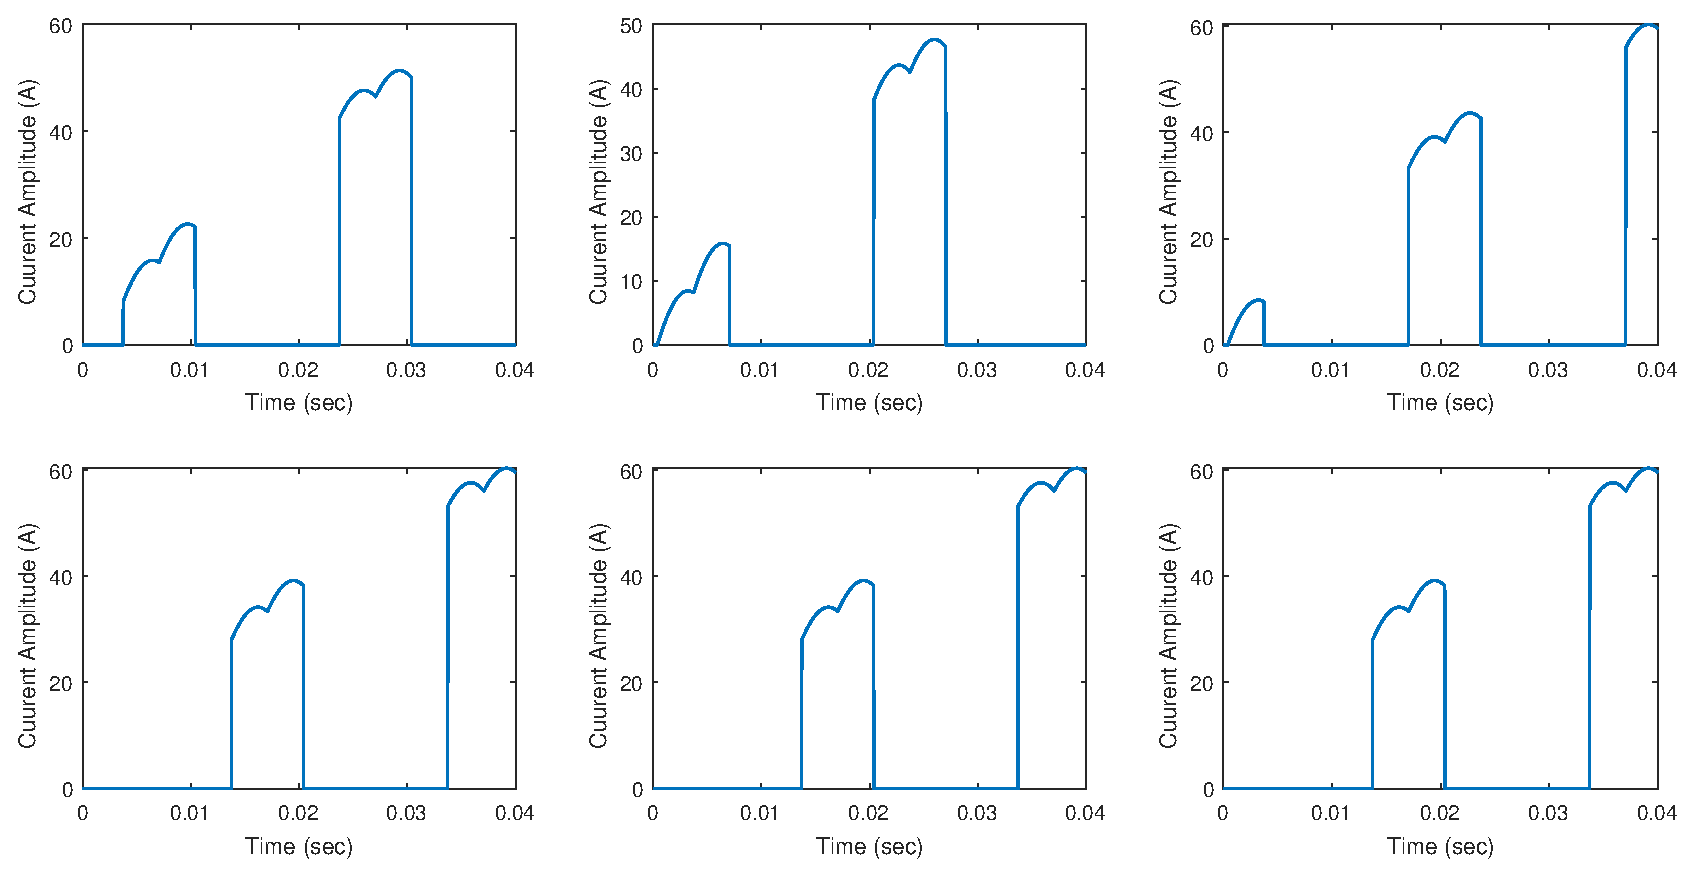
\includegraphics[width = 0.9\textwidth]{Images/3_ThI_67_08}
		\caption{a = 67, L = 0.08}
		\label{fig:3_ThI_67_08}
	\end{subfigure}
	\caption{Thyristor Currents (a=67 L=0.04/0.08)}
	\label{figs:3_ThI_67}
\end{figure}
Το figures \ref{figs:3_ThI_67} αναπαριστούν το ρεύμα σε κάθε Thyristor για χρόνο 2 περιόδων. Το ρεύμα της διόδου είναι ίσο με το ρεύμα εξόδου όταν αυτή άγει εφόσον θεωρούνται ιδανικές. Οι δίοδοι άγουν σύμφωνα με τον πίνακα της υποενότητας.....
